\documentclass[letterpaper]{article}
\usepackage{geometry}
\geometry{margin=1.1in}
\usepackage[protrusion=true,expansion=true]{microtype}	
\usepackage[boxruled,linesnumbered,vlined,inoutnumbered]{algorithm2e}
\usepackage{amsmath}
\usepackage{amsthm}
\usepackage{amssymb}
\usepackage{mathtools}
\usepackage{mathrsfs}
\usepackage{soul}
\usepackage{natbib}
\usepackage[table]{xcolor}
\usepackage{rotating}
\usepackage{gensymb}
\usepackage{lscape}
\usepackage{array}
\usepackage{makecell}
\renewcommand\theadalign{bc}
\renewcommand\theadfont{\bfseries}
\renewcommand\theadgape{\Gape[4pt]}
\renewcommand\cellgape{\Gape[4pt]}
\usepackage{courier}
\usepackage{lipsum}
\usepackage{graphicx}
\usepackage{subcaption}
\usepackage[space]{grffile}
\usepackage{xcolor}
\definecolor{light-grey}{rgb}{0.9,0.9,0.9}
\definecolor{dark-red}{rgb}{0.4,0.15,0.15}
\definecolor{dark-blue}{rgb}{0,0,0.7}
\usepackage{environ}
\setcounter{tocdepth}{2}
\renewcommand{\contentsname}{Table of Contents}
\usepackage{hyperref}
\hypersetup{
    colorlinks, linkcolor={dark-blue},
    citecolor={dark-blue}, urlcolor={dark-blue}
}

\setlength{\parskip}{1em}
\newcommand{\HIGHLIGHT}[1]{\textcolor{blue}{\textbf{#1}}}
\newcommand{\TODO}[1]{\textcolor{red}{\textbf{#1}}}

\begin{document}
%-----------------
%	Homework 4
%-----------------
\newpage
\section*{Calvin Cuff}
\begin{center}
    \begin{Large}
    COMPSCI 589 - Final Project - Spring 2025
    \end{Large}
    \\
    \HIGHLIGHT{Due May 9, 2025, 11:59 pm Eastern Time}
\end{center}

\section{Final Project — Overall Goals}

\begin{itemize}
  \item The goal of this final project is to compare the performance of different machine learning algorithms
you implemented throughout the semester by testing them on four new, challenging datasets.
  \item By performing these comparisons, you will gain practical experience in selecting an algorithm (based on
a given problem) and optimizing its hyper-parameters so that it works well. In addition, these analyses
will give you insight into how to solve novel machine learning problems—problems where no one tells
you which algorithms may work best nor how to adjust their hyper-parameters.
\end{itemize}


\section{The Hand-Written Digits Recognition Dataset}
The goal, here, is to analyze 8x8 pictures of hand-written digits and classify them as belonging to one of 10 possible classes. Each class is associated with one particular digit: 0, 1, . . . , 9. In this dataset, each instance is composed of 8 × 8 = 64 numerical attributes, each of which corresponding to the grayscale value of one pixel in the image being classified. This dataset is composed of 1797 instances.

For the Sklearn digits I chose to evaluate \textbf{k Nearest Neighbors} and \textbf{Random Forests} algorithms. The dataset is considerably small and the images themselves are of low dimensionality (8x8) so a KNN algorithm should perform well in terms of runtime performance. The image classes are also well separated so the raw pixel differences should be a good indicator of class membership. Random Forests use an ensemble of Decision Trees so this algorithm should be well suited for classification as they are less sensitive to noise in the data. By their random nature and majority voting, the model should be able to determine which pixels contribute the most to digit classification.

\subsection{KNN Hyper Parameter Search Results}

    Hyper parameter search was performed across a varying number of k neighbors (1, 3, 5, 7, 9, 11, 13, 21, 35, 51) to identify the optimal settings. These experiments used stratified cross validation, using 10 folds.

\begin{table}[h]
\centering
\begin{tabular}{|c|c|c|}
\hline
\textbf{k} & \textbf{Mean Accuracy} & \textbf{Mean F1 Score} \\
\hline
1  & 0.9847 & 0.9316 \\
\textbf{3}  & \textbf{0.9861} & \textbf{0.9370} \\
5  & 0.9854 & 0.9334 \\
7  & 0.9840 & 0.9275 \\
9  & 0.9805 & 0.9140 \\
11 & 0.9805 & 0.9143 \\
13 & 0.9770 & 0.9004 \\
21 & 0.9729 & 0.8840 \\
35 & 0.9548 & 0.8131 \\
51 & 0.9437 & 0.7722 \\
\hline
\end{tabular}
\caption{KNN Performance on Digits Dataset: Accuracy and F1 Score Across Different k Values}
\label{tab:knn_results}
\end{table}

Following the prior stratified cross validation experiments, the optimal hyper parameter setting for the number of nearest neighbors was shown to be 3. Using this setting allowed the KNN model to achieve its highest accuracy (98.61\%) and F1 Score (0.9370).

 \vspace{0.2in}
        \begin{minipage}{\linewidth}
            \centering
            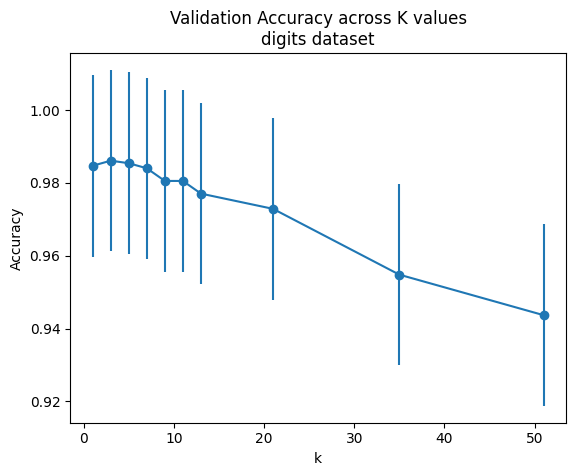
\includegraphics[width=10cm]{figures/digits-knn-val-accuracies.png}
            \captionof{figure}{KNN Performance on Digits Dataset Across k values}
        \end{minipage}
\vspace{0.1in}

\subsection*{KNN Results}
The graph shows validation accuracy across different values of k using 10-fold cross-validation. Overall, KNN performs very well on this dataset, with accuracy remaining high (~>97\%) for most values of k. The best performance is observed for smaller values of k (around 3–5), where the model best identifies the class separation in the pixel space. As k increases beyond 20, accuracy gradually declines, indicating digits from other classes may have similar pixel distances and start being included as nearest neighbors.


\subsection{Random Forest Hyper Parameter Search Results}

 Hyper parameter search was performed across a varying number of decision trees that compose a Random Forest (1, 5, 10, 20, 30, 40, 50) to identify the optimal settings. These experiments used stratified cross validation, using 10 folds.

 \begin{table}[h]
\centering
\begin{tabular}{|c|c|c|}
\hline
\textbf{Number of Trees (n\_tree)} & \textbf{Mean Accuracy} & \textbf{Mean F1 Score} \\
\hline
1  & 0.7383 & 0.3361 \\
5  & 0.8963 & 0.6405 \\
10 & 0.9367 & 0.7600 \\
20 & 0.9541 & 0.8159 \\
30 & 0.9631 & 0.8448 \\
40 & 0.9589 & 0.8282 \\
\textbf{50} & \textbf{0.9659} & \textbf{0.8567} \\
\hline
\end{tabular}
\caption{Random Forest Performance on Digits Dataset: Accuracy and F1 Score Across Varying Tree Counts}
\label{tab:rf_ntree_results}
\end{table}

Following the prior stratified cross validation experiments, the optimal hyper parameter setting for the
number of Decision Trees in a Random Forest was shown to be 50. Using this setting allowed the Random Forest model to achieve its highest accuracy (96.59\%) and F1 Score (0.8567).

\vspace{0.2in}
    \begin{minipage}{\linewidth}
        \centering
        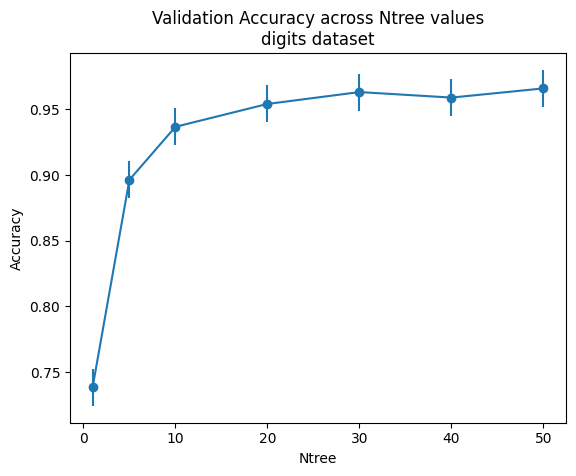
\includegraphics[width=10cm]{figures/digits-rf-ntree-val-accuracies.png}
        \captionof{figure}{Random Forest Performance on Digits Dataset Across number of trees}
    \end{minipage}
\vspace{0.1in}

\subsection*{Random Forest Results}

The graph shows how validation accuracy varies with the number of trees (ntree) in a Random Forest classifier. The model improves substantially with just a small number of trees, increasing from ~74\% accuracy at ntree = 1 to ~90\% at ntree = 5. Accuracy continues to improve more gradually as more trees are added. Performance begins to plateau around ntree = 30, suggesting diminishing returns beyond that point. The performance gain from increasing ntree illustrates the ensemble’s ability to combine diverse weak learners via bootstrapped subsets and random feature splits into a strong overall model.

\clearpage

\section{The Oxford Parkinson’s Disease Detection Dataset}
This dataset is composed of a range of biomedical voice measurements from 31 people, 23 of whom are patients with Parkinson’s disease. Each row in the dataset corresponds to the voice recording from one of these individuals. Each attribute corresponds to the measurement of one specific property of the patient’s voice—for example, their average vocal frequency or several measures of frequency variation. The goal, here, is to predict whether a particular person is healthy or whether it is a patient with Parkinson’s. The binary target class to be predicted is Diagnosis: whether the patient is healthy (class 0) or a patient with Parkinson’s (class 1). There are 195 instances in this dataset. All 22 attributes are numerical. The Parkinson’s dataset can be found in this assignment’s zip file on Canvas.

For the Parkinson’s dataset, I selected to evaluate \textbf{Decision Trees} and a \textbf{Neural Network}. Decision Trees should be able to help identify potential non-linear relationships and give insight into which features are the most informative for class detection. Neural networks were also explored due to their flexibility in modeling complex patterns, using techniques like regularization to minimize overfitting on the smaller dataset.

\subsection{Decision Tree Hyper Parameter Search Results}

    Hyper parameter search was performed across a varying number of stop criteria to identify the optimal settings for a Decision Tree. These stop criteria included a Maximal Depth of [5,15], a Minimal Information Gain of [0.1, 0.01], and a Minimal Split Size of [5,11].   
    These experiments used stratified cross validation, using 10 folds.

\begin{table}[h]
\centering
\begin{tabular}{|l|c|c|}
\hline
\textbf{Stop Criterion} & \textbf{Mean Accuracy} & \textbf{Mean F1 Score} \\
\hline
MaximalDepth(5)             & 0.8331 & 0.8922 \\
MaximalDepth(15)            & 0.7891 & 0.8625 \\
MinimalGain(0.1)            & 0.7823 & 0.8750 \\
\textbf{MinimalGain(0.01)}  & \textbf{0.8526} & \textbf{0.9028} \\
MinimalSizeForSplit(5)      & 0.8526 & 0.9022 \\
MinimalSizeForSplit(11)     & 0.8018 & 0.8658 \\
\hline
\end{tabular}
\caption{Decision Tree Performance on the Parkinson's Dataset Across Different Stopping Criteria}
\label{tab:dt_parkinsons_results}
\end{table}


Following the prior stratified cross validation experiments, the optimal hyper parameter setting for the stop criteria of a Decision Tree when predicting classes of the Parkinsons dataset was Minimal Information Gain at 0.01. Using this setting allowed the Decision Tree model to achieve its highest accuracy (85.26\%) and F1 Score (0.9028).

\subsection*{Best Decision Tree Test Accuracy}

Deploying the Decision Tree with the optimal hyper parameter settings identified as Minimal Gain at 0.01, the model was trained over 100 iterations, measuring the test accuracy after each iteration. The following graph highlights the distribution of the test accuracy.

\vspace{0.2in}
    \begin{minipage}{\linewidth}
        \centering
        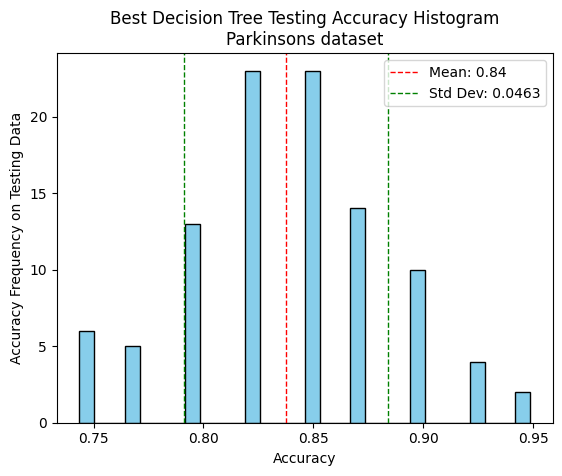
\includegraphics[width=10cm]{figures/best_dt_parkinsons_testing_hist.png}
        \captionof{figure}{Decision Tree Test Performance on Parkinsons Dataset}
    \end{minipage}
\vspace{0.1in}


The results show a distribution centered around a mean accuracy of 0.84, with a standard deviation of 0.0463. Most accuracy values fall between approximately 0.80 and 0.89, indicating that the model's generalization performance is both stable and reliable across different iterations. This behavior suggests the Decision Tree captures consistent patterns in the input features without overfitting, despite the relatively small size and possible noise in the Parkinson’s data. The histogram also visually reinforces that this configuration balances complexity and generalization effectively.

\subsection{Neural Network Hyper Parameter Search Results}

    Hyper parameter search was performed across a varying number of network architectures to identify the optimal settings for a Neural Network. For the experiments, I varied the learning rate (1e-3, 1e-2, 5e-2, 1e-1, 5e-1), the regularization strength (0.0, 1e-3, 1e-2, 1e-1), and the size of hidden dimensions in the network ([2], [2,2], [2,2,2], [10], [10,10], [20], [40], [20,10], [30,15], [40,20,10]). This resulted in a total of 200 different network permutations, only the top 10 configurations are shown here. These experiments used stratified cross validation, using 10 folds.


     \vspace{0.2in}
        \begin{minipage}{\linewidth}
            \centering
            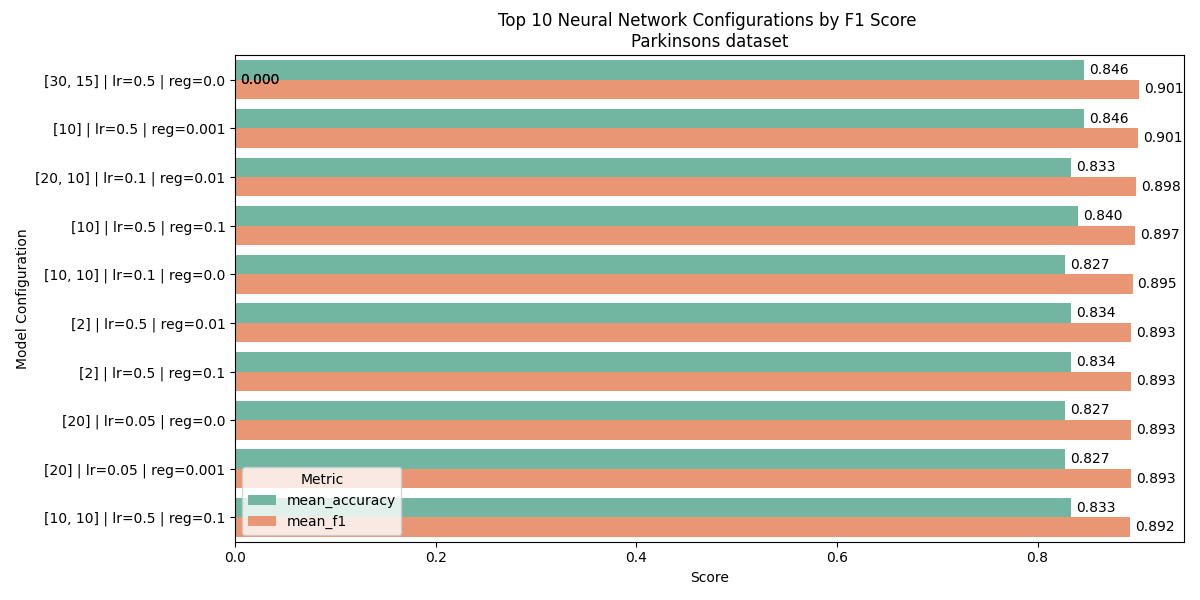
\includegraphics[width=15cm]{figures/parkinsons-nn-results.png}
            \captionof{figure}{Neural Network Perfomance on the Parkinson's Dataset Across Different Hyper Parameters}
        \end{minipage}
    \vspace{0.1in}
    
Following the prior stratified cross validation experiments, the optimal hyper parameter settings for  a Neural Network when predicting classes of the Parkinson's dataset was a learning rate of 0.5, no regularization, and hidden dimensions of [30,15]. Using these parameters allowed the Neural Network to achieve its highest accuracy (84.6\%) and F1 Score (0.901).

\clearpage
\subsection*{Best Neural Network Loss}

Deploying the best Neural Network architecture previously identified the model was trained iteratively on a number of training samples, measuring the test loss after each epoch.

\vspace{0.2in}
        \begin{minipage}{\linewidth}
            \centering
            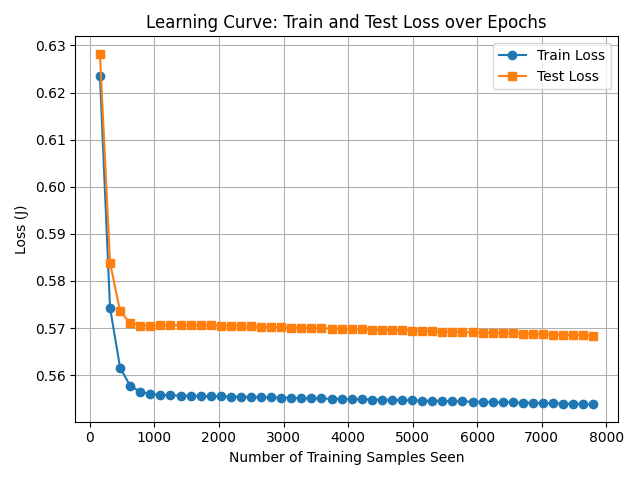
\includegraphics[width=10cm]{figures/best_nn_parkinsons_loss_curve.png}
            \captionof{figure}{Neural Network Train/Test Loss Curve over 50 epochs}
        \end{minipage}
    \vspace{0.1in}

The plot illustrates a rapid decrease in both training and test loss during the initial epochs, eventually leveling off. Training loss continues to decline gradually, while test loss stabilizes early, suggesting the model generalizes well without overfitting. The gap between the curves remains small, indicating that the network is not memorizing the training data and maintains a consistent generalization margin. This curve confirms that the selected architecture is well-tuned for the dataset’s size and complexity, and it effectively models the relationship between features and class labels in the Parkinson’s data.

\clearpage

\section{The Rice Grains Dataset}

This dataset contains information about 3810 rice grain images. In particular, each rice grain instance is described by 7 numerical morphological features that were inferred from images of different rice grains (e.g., the longest line that can be drawn on the rice grain). The goal is to predict whether a given rice grain belongs to the Cammeo species or the Osmancik species. This dataset can be found in this assignment’s zip file on Canvas.

 For the Rice Grains dataset, I chose to evaluate  \textbf{k Nearest Neighbors} and a \textbf{Decision Tree} classifier. KNN was chosen due to the spatial nature of the features, which makes Euclidean distance a meaningful similarity measure. Decision Trees were used to capture potentially nonlinear interactions between grain attributes while maintaining interpretability. Both models were evaluated under various hyperparameter settings to identify optimal configurations.

\subsection{KNN Hyper Parameter Search Results}

    Hyper parameter search was performed across a varying number of k neighbors (1, 3, 5, 7, 9, 11, 13, 21, 35, 51, 65) to identify the optimal settings. These experiments used stratified cross validation, using 10 folds.

\begin{table}[h]
\centering
\begin{tabular}{|c|c|c|}
\hline
\textbf{k} & \textbf{Mean Accuracy} & \textbf{Mean F1 Score} \\
\hline
1   & 0.8888 & 0.9023 \\
3   & 0.9121 & 0.9233 \\
5   & 0.9229 & 0.9329 \\
7   & 0.9278 & 0.9370 \\
9   & 0.9278 & 0.9370 \\
11  & 0.9262 & 0.9356 \\
13  & 0.9285 & 0.9377 \\
21  & 0.9272 & 0.9365 \\
35  & 0.9281 & 0.9372 \\
\textbf{51}  & \textbf{0.9321} & \textbf{0.9407} \\
65  & 0.9308 & 0.9396 \\
\hline
\end{tabular}
\caption{KNN Performance on the Rice Grains Dataset Across Different Values of k}
\label{tab:knn_rice_results}
\end{table}

Following the prior stratified cross validation experiments, the optimal hyper parameter setting for the number of nearest neighbors was shown to be 51. Using this setting allowed the KNN model to achieve its highest accuracy (93.21\%) and F1 Score (0.9407).


\vspace{0.2in}
    \begin{minipage}{\linewidth}
        \centering
        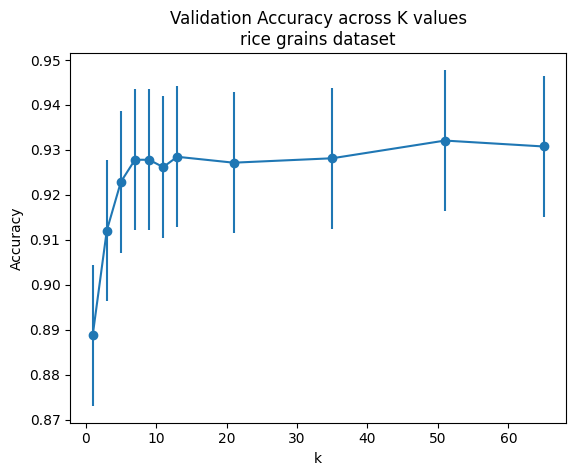
\includegraphics[width=10cm]{figures/grains-knn-val-accuracies.png}
        \captionof{figure}{KNN Performance on Rice Grains Across k values}
    \end{minipage}
\vspace{0.1in}

\subsection*{KNN Results}

The validation accuracy plot for KNN on the rice grains dataset demonstrates strong overall performance, with accuracy improving rapidly at low k values and stabilizing around k = 5 to 13. Accuracy peaks slightly above 93\% and remains consistent across larger values of k, indicating that the model maintains high generalization regardless of slight increases in the number of neighbors. The initial improvement reflects the model's ability to identify patterns in class features by including additional neighbors. Beyond a certain point, adding more neighbors offers diminishing returns, as the decision boundaries become smoother. This trend indicates that the rice dataset has clearly separable class features that KNN can effectively capture with moderate neighborhood sizes.



\subsection{Decision Tree Hyper Parameter Search Results}

    Hyper parameter search was performed across a varying number of stop criteria to identify the optimal settings for a Decision Tree. These stop criteria included a Maximal Depth of [5,15], a Minimal Information Gain of [0.1, 0.01], and a Minimal Split Size of [5,11].   
    These experiments used stratified cross validation, using 10 folds.


\begin{table}[h]
\centering
\begin{tabular}{|l|c|c|}
\hline
\textbf{Stop Criterion} & \textbf{Mean Accuracy} & \textbf{Mean F1 Score} \\
\hline
MaximalDepth(5)    & 0.9094 & \textbf{0.9213} \\
MaximalDepth(15)            & 0.8674 & 0.8837 \\
MinimalGain(0.1)            & \textbf{0.9107} & 0.9192 \\
MinimalGain(0.01)           & 0.8832 & 0.8972 \\
MinimalSizeForSplit(5)      & 0.8753 & 0.8890 \\
MinimalSizeForSplit(11)     & 0.8989 & 0.9113 \\
\hline
\end{tabular}
\caption{Decision Tree Performance on the Rice Grains Dataset Across Different Stopping Criteria}
\label{tab:dt_rice_results}
\end{table}

Following the prior stratified cross validation experiments, the optimal hyper parameter setting for the stop criteria of a Decision Tree when focused o the accuracy of the Rice Grains dataset was Minimal Information Gain at 0.1. Using this setting allowed the Decision Tree model to achieve its highest accuracy (91.07\%). The stopping criteria that allowed the model to achieve its highest F1 score was a stopping criteria of a Maximal Depth of 5, with F1 Score of 0.9213.

\subsection*{Best Decision Tree Test Accuracy}

Deploying the Decision Tree with the optimal hyper parameter settings identified as Maximal Depth of 5, the model was trained over 100 iterations, measuring the test accuracy after each iteration. The following graph highlights the distribution of the test accuracy.

\vspace{0.2in}
    \begin{minipage}{\linewidth}
        \centering
        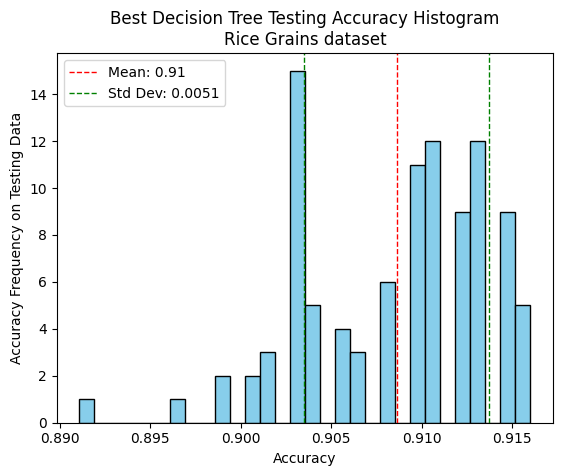
\includegraphics[width=10cm]{figures/best_dt_grains_testing_hist.png}
        \captionof{figure}{Decision Tree Test Performance on Rice Grains Dataset}
    \end{minipage}
\vspace{0.1in}

The model exhibits very stable performance, with a mean accuracy of 0.91 and a standard deviation of just 0.0051. The distribution is centered around the mean, with most runs achieving accuracy between 0.905 and 0.915. This consistency suggests that the model generalizes reliably across the dataset and that the chosen depth constraint effectively prevents overfitting while maintaining high accuracy. The structured and separated feature space in the rice grains dataset likely contributes to the model’s ability to make accurate predictions.


\clearpage

\section{ The Credit Approval Dataset}

This dataset contains information about 653 credit card applications. Attribute names and their values were mapped from their original representation to one that is not easily interpretable by humans to protect the confidentiality of the data; that said, they still do contain all necessary information to construct effective classifiers. The goal is to predict whether a given credit card application would be approved or not. Each
credit card application is described by 6 numerical features and 9 categorical features. This dataset can be found in this assignment’s zip file on Canvas.

For classifying instances from the Credit Aproval dataset I chose to use a \textbf{Random Forest} and \textbf{Neural Network}. Random Forests are well-suited for handling both numerical and categorical features without requiring extensive preprocessing, and they are robust to noise and overfitting due to their ensemble structure. Neural Networks are capable of modeling complex, non-linear relationships between features. With proper normalization and one-hot encoding, they can effectively learn from mixed-type inputs and provide a high-capacity alternative to tree-based models. 

\subsection{Random Forest Hyper Parameter Search Results}

 Hyper parameter search was performed across a varying number of decision trees that compose a Random Forest (1, 5, 10, 20, 30, 40, 50, 100) to identify the optimal settings. These experiments used stratified cross validation, using 10 folds.

 \begin{table}[h]
\centering
\begin{tabular}{|c|c|c|}
\hline
\textbf{Number of Trees} & \textbf{Mean Accuracy} & \textbf{Mean F1 Score} \\
\hline
1    & 0.8278 & 0.8136 \\
5    & 0.8354 & 0.8179 \\
10   & 0.8411 & 0.8268 \\
20   & 0.8563 & 0.8415 \\
30   & 0.8469 & 0.8360 \\
40   & 0.8545 & 0.8429 \\
50   & 0.8488 & 0.8367 \\
\textbf{100}  & \textbf{0.8603} & \textbf{0.8505} \\
\hline
\end{tabular}
\caption{Random Forest Performance on the Credit Loan Dataset Across Different Tree Counts}
\label{tab:rf_creditloan_results}
\end{table}

Following the prior stratified cross validation experiments, the optimal hyper parameter setting for the number of Decision Trees in a Random Forest was shown to be 100. Using this setting allowed the Random Forest model to achieve its highest accuracy (86.03\%) and F1 Score (0.8505).


\vspace{0.2in}
\begin{minipage}{\linewidth}
    \centering
    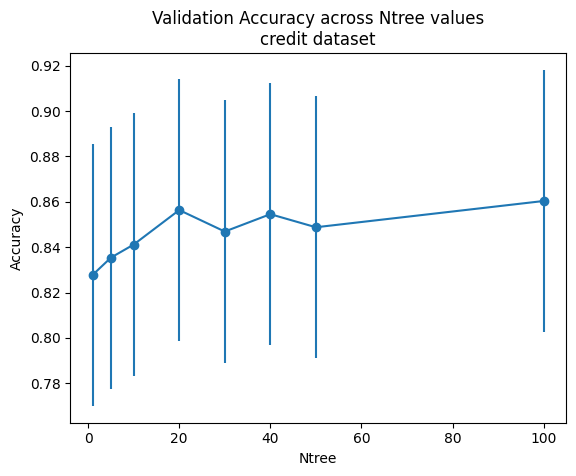
\includegraphics[width=10cm]{figures/credit-rf-ntree-val-accuracies.png}
    \captionof{figure}{Random Forest Performance on Credit Dataset Across number of trees}
\end{minipage}
\vspace{0.1in}

\subsection*{Random Forest Results}

The validation accuracy curve shows a gradual improvement in performance as the number of trees increases. Accuracy improves steadily from ntree = 1 up to about ntree = 20, after which performance fluctuates slightly but remains within a consistent range. By ntree = 100, the model reaches its best result, though with relatively wide error bars indicating some variability across folds. Due to the moderate size and mixed data types of the credit dataset, returns diminish beyond a certain point, and gains are less pronounced compared to simpler or more structured datasets.


\subsection{Neural Network Hyper Parameter Search Results}

    Hyper parameter search was performed across a varying number of network architectures to identify the optimal settings for a Neural Network. For the experiments, I varied the learning rate (1e-3, 1e-2, 5e-2, 1e-1, 5e-1), the regularization strength (0.0, 1e-3, 1e-2, 1e-1), and the size of hidden dimensions in the network ([2], [2,2], [2,2,2], [10], [10,10], [20], [40], [20,10], [30,15], [40,20,10]). This resulted in a total of 200 different network permutations, only the top 10 configurations are shown here. These experiments used stratified cross validation, using 10 folds.


     \vspace{0.2in}
        \begin{minipage}{\linewidth}
            \centering
            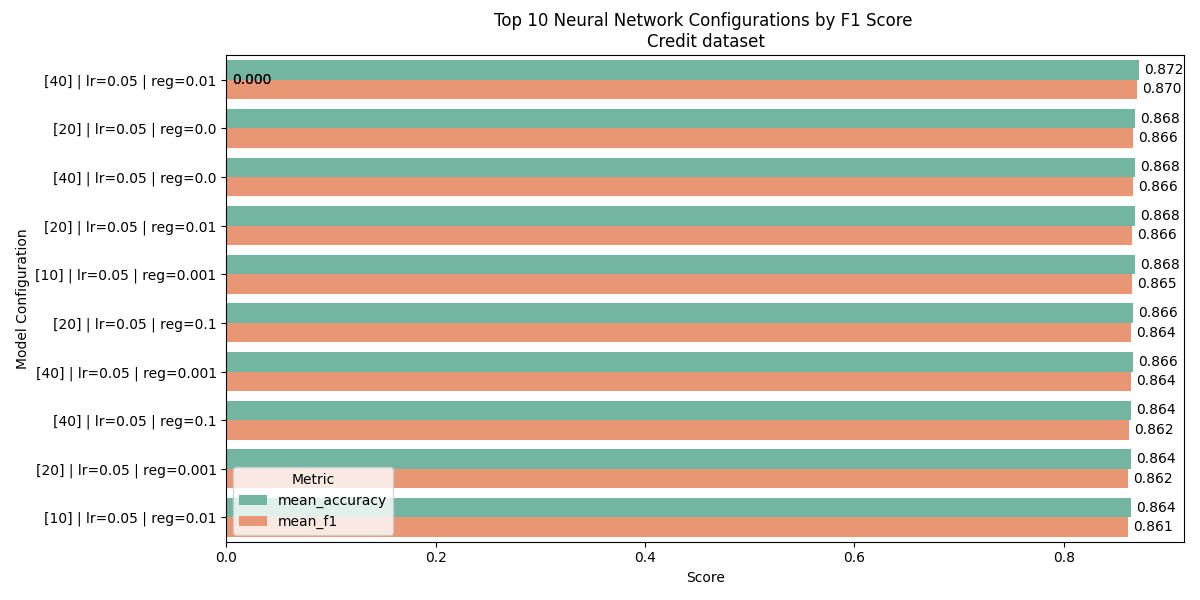
\includegraphics[width=15cm]{figures/credit-nn-results.png}
            \captionof{figure}{Neural Network Perfomance on the Credit Loan Dataset Across Different Hyper Parameters}
        \end{minipage}
    \vspace{0.1in}
    
Following the prior stratified cross validation experiments, the optimal hyper parameter settings for  a Neural Network when predicting classes of the Parkinson's dataset was a learning rate of 0.05, regularization strength of 0.01, and hidden dimensions of [40]. Using these parameters allowed the Neural Network to achieve its highest accuracy (87.2\%) and F1 Score (0.870).

\clearpage
\subsection*{Best Neural Network Loss}

Deploying the best Neural Network architecture previously identified the model was trained iteratively on a number of training samples, measuring the test loss after each epoch.

\vspace{0.2in}
    \begin{minipage}{\linewidth}
        \centering
        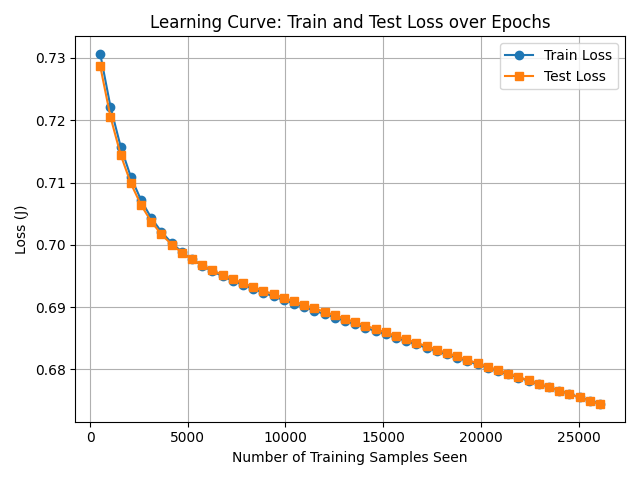
\includegraphics[width=10cm]{figures/best_nn_credit_loss_curve.png}
        \captionof{figure}{Neural Network Train/Test Loss Curve over 50 epochs}
    \end{minipage}
\vspace{0.1in}

The model shows consistent improvement over time, with both training and test loss decreasing steadily in parallel. The similar shape of the two curves throughout training indicates that the model is generalizing well and not overfitting. The smooth, gradual descent suggests that the learning rate and regularization were well tuned, allowing for stable convergence. The neural network demonstrates strong and stable learning behavior on the credit loan dataset, successfully minimizing loss on unseen data while preserving generalization across epochs.


\section{Results Summary}
% Please add the following required packages to your document preamble:
% \usepackage[table,xcdraw]{xcolor}
% Beamer presentation requires \usepackage{colortbl} instead of \usepackage[table,xcdraw]{xcolor}
% Please add the following required packages to your document preamble:
% \usepackage[table,xcdraw]{xcolor}
% Beamer presentation requires \usepackage{colortbl} instead of \usepackage[table,xcdraw]{xcolor}
\begin{table}[h]
\begin{tabular}{|c|cc|cc|cc|cc|}
\hline
               & \multicolumn{2}{c|}{Digits}                                                          & \multicolumn{2}{c|}{Parkinsons}                                                    & \multicolumn{2}{c|}{Rice Grains}                                                     & \multicolumn{2}{c|}{Credit Loan}                                                     \\ \hline
               & \multicolumn{1}{c|}{Accuracy}                       & F1-Score                       & \multicolumn{1}{c|}{Accuracy}                      & F1-Score                      & \multicolumn{1}{c|}{Accuracy}                       & F1-Score                       & \multicolumn{1}{c|}{Accuracy}                       & F1-Score                       \\ \hline
KNN            & \multicolumn{1}{c|}{\cellcolor[HTML]{9B9B9B}0.9861} & \cellcolor[HTML]{9B9B9B}0.9370 & \multicolumn{1}{c|}{\cellcolor[HTML]{FFFFFF}}      & \cellcolor[HTML]{FFFFFF}      & \multicolumn{1}{c|}{\cellcolor[HTML]{9B9B9B}0.9321} & \cellcolor[HTML]{9B9B9B}0.9407 & \multicolumn{1}{c|}{\cellcolor[HTML]{FFFFFF}}       & \cellcolor[HTML]{FFFFFF}       \\ \hline
Decision Tree  & \multicolumn{1}{c|}{\cellcolor[HTML]{FFFFFF}}       & \cellcolor[HTML]{FFFFFF}       & \multicolumn{1}{c|}{\cellcolor[HTML]{9B9B9B}0.85}  & \cellcolor[HTML]{FFFFFF}0.90  & \multicolumn{1}{c|}{\cellcolor[HTML]{FFFFFF}0.91}   & \cellcolor[HTML]{FFFFFF}0.92   & \multicolumn{1}{c|}{\cellcolor[HTML]{FFFFFF}}       & \cellcolor[HTML]{FFFFFF}       \\ \hline
Random Forest  & \multicolumn{1}{c|}{\cellcolor[HTML]{FFFFFF}0.9659} & \cellcolor[HTML]{FFFFFF}0.8567 & \multicolumn{1}{c|}{\cellcolor[HTML]{FFFFFF}}      & \cellcolor[HTML]{FFFFFF}      & \multicolumn{1}{c|}{\cellcolor[HTML]{FFFFFF}}       & \cellcolor[HTML]{FFFFFF}       & \multicolumn{1}{c|}{\cellcolor[HTML]{FFFFFF}0.8603} & \cellcolor[HTML]{FFFFFF}0.8505 \\ \hline
Neural Network & \multicolumn{1}{c|}{\cellcolor[HTML]{FFFFFF}}       & \cellcolor[HTML]{FFFFFF}       & \multicolumn{1}{c|}{\cellcolor[HTML]{FFFFFF}0.846} & \cellcolor[HTML]{9B9B9B}0.901 & \multicolumn{1}{c|}{\cellcolor[HTML]{FFFFFF}}       & \cellcolor[HTML]{FFFFFF}       & \multicolumn{1}{c|}{\cellcolor[HTML]{9B9B9B}0.872}  & \cellcolor[HTML]{9B9B9B}0.870  \\ \hline
\end{tabular}
\end{table}

\end{document}